\begin{itemize}
\item Case law: made up of, and from, hundred and thousands of precedent cases
\item Principle: cases with similar facts should be treated in similar ways 
\item In cases where the parties disagree on what the law is: looking to past precedential decisions of relevant courts
\item If a similar dispute has been resolved in the past: following the reasoning used in the prior decision
\item If the current dispute is fundamentally distinct from all previous cases: creating new 
\item CBR: analogous to human experts solving a problem through employing their relevant past experience
\begin{itemize}
\item exemplar-based reasoning
\item instance-based reasoning
\item memory-based reasoning
\item case-based reasoning
\item analogy-based reasoning
\end{itemize}
\item if the new problem has some novel aspects, aspects, then the solution to the new problem is added to the case base
\item Different from diagnostic fault tree or rule-based system
\begin{itemize}
\item memory-based problem-solving
\item reusing past experiences
\end{itemize}
\end{itemize}

Domains that CBR Works well:
\begin{itemize}
\item Broad but shallow domain
\begin{itemize}
\item not a single tree, but a forest of small trees
\item a number of loosely connected problems that must be dealt with
\item need different kinds of expertise
\end{itemize}
\item Experience, rather than theory, is the primary source of knowledge
\begin{itemize}
\item Many past examples of problems that occur
\item rather than having a deep understanding of the domain
\end{itemize}
\item solutions are reusable
\begin{itemize}
\item old solution is useful for a new problem
\item if each problem is different, then there is little to be gained by trying to reuse past solutions
\end{itemize}
\end{itemize}

\section{Case-Based Reasoning System and 4R Cycle}
\begin{itemize}
\item Input: new problem
\item Output: a solution to the new problem
\item case base
\begin{itemize}
\item store cases(experience)
\end{itemize}
\end{itemize}

\begin{figure}[h]
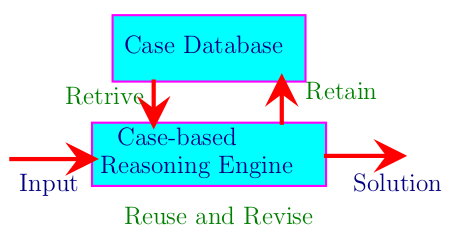
\includegraphics[scale=1]{chap7_pics/case_base_sys.png} 
\caption{The Case-Based Reasoning System}
\end{figure}


\subsection{4R Cycle}

\begin{figure}[h]
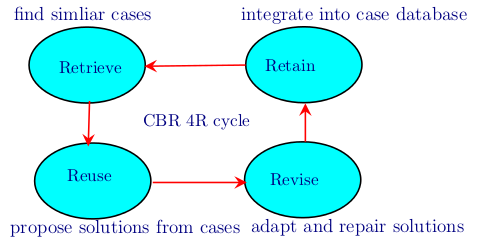
\includegraphics[scale=1]{chap7_pics/case-base-4rcycle.png} 
\caption{The Case-Based 4R cycle}
\label{case-base_4rcycle}
\end{figure}

\begin{itemize}
\item Retrieve: relevant cases, match most similar cases, retrieve solutions from theses cases
\item Reuse: solutions in stored cases
\item Revise: the retrieved solution(s) to reflect differences between new case and retrieved case(s)
\item Retain: new cases into database
\end{itemize}

See figure\ref{case-base_4rcycle} for visualisation.

\subsubsection{New Problem vs Old Case}
\begin{itemize}
\item Observations define a new problem
\item Compare similarity of each feature
\item Not all feature values may be known
\item Some features may be more important
\item New problem = case without a solution
\item Similarity by weighted average
\end{itemize}

\section{Design Case-Based Reasoning System}
\subsection{Case Representation}
A case in diagnosis represents one diagnostic situation, include two parts:\\
\begin{enumerate}
\item Features
\begin{enumerate}
\item symptoms
\item failure
\item feature values
\item repair strategies
\item test time and cost
\end{enumerate}
\item Solutions
\begin{enumerate}
\item cause of failure
\item replace or repair fault unit
\end{enumerate}
\end{enumerate}

\subsection{Design Case database}
\begin{itemize}
\item Dependent on the structure and content of its collection of cases
\begin{itemize}
\item Deciding what to store in a case
\item Finding an appropriate structure for describing case contents
\item Deciding how the case memory should be organized and indexed for effective retrieval and reuse
\end{itemize}
\end{itemize}

\subsection{Retrieve: index}
\begin{itemize}
\item Retrieve a case from case database
\item Select indexes
\begin{itemize}
\item Similar to books in library, index may help search cases in case database
\end{itemize}
\end{itemize}

\subsubsection{Match Case}
\begin{itemize}
\item Compare features and their value between the stored case and new problem
\item Nearest-neighbour matching algorithm
\end{itemize}

\subsection{Retrieval: Ranking}
\begin{itemize}
\item Possibly more than one case is matched
\item Among matched cases, ranking may be used to choose a case to reuse
\item If a matched case cannot provide the solution to the problem,. lower rank cases may be taken as the candidate for the problem
\item Ranking value will depend on observation time and cost
\begin{itemize}
\item Higher the rank $\longrightarrow$ better solution(cheaper, faster, etc.)
\item Ranking Observation cost, observation time and case frequency need to be considered
\end{itemize}
\end{itemize}

\subsection{Reuse/Revive}
\begin{itemize}
\item Adapt/repair old solutions
\item Different approaches
\begin{itemize}
\item Substitution
\item Parameter adjustment(via specialized heuristics, e.g. Judge)
\item Local search(replacing fruits in a recipe)
\item Special purpose adaptation and repair
\item Model-based
\end{itemize}
\end{itemize}

\subsection{Retain: Store new cases and stop reasoning}
\begin{itemize}
\item Store all new cases
\item Or store selected new cases(based on certain criteria?)
\item The reasoning stops until a satisfied solution(from a solved case) is found
\item or stop the reasoning procedure by the system
\end{itemize}
